\documentclass[article,dr=phil,type=msc,colorback,accentcolor=tud9c]{tudthesis}

\usepackage[english]{babel}
\usepackage{listings}
\usepackage{color}
\usepackage{verbatim}
\usepackage{appendix} 
\usepackage{url}

\definecolor{mygreen}{rgb}{0,0.6,0}
\definecolor{mygray}{rgb}{0.5,0.5,0.5}
\definecolor{mymauve}{rgb}{0.38,0,0.38}

\lstset{ 
	backgroundcolor=\color{white},   % choose the background color; you must add \usepackage{color} or \usepackage{xcolor}; should come as last argument
	basicstyle=\footnotesize,        % the size of the fonts that are used for the code
	breakatwhitespace=false,         % sets if automatic breaks should only happen at whitespace
	breaklines=true,                 % sets automatic line breaking
	captionpos=b,                    % sets the caption-position to bottom
	commentstyle=\color{mygreen},    % comment style
	deletekeywords={...},            % if you want to delete keywords from the given language
	escapeinside={\%*}{*)},          % if you want to add LaTeX within your code
	extendedchars=true,              % lets you use non-ASCII characters; for 8-bits encodings only, does not work with UTF-8
	frame=single,	                   % adds a frame around the code
	keepspaces=true,                 % keeps spaces in text, useful for keeping indentation of code (possibly needs columns=flexible)
	keywordstyle=\bfseries\color{mymauve},       % keyword style
	language=Java,                 % the language of the code
	morekeywords={*,get,await,deposit,deduct,interface},            % if you want to add more keywords to the set
	numbers=left,                    % where to put the line-numbers; possible values are (none, left, right)
	numbersep=5pt,                   % how far the line-numbers are from the code
	numberstyle=\tiny\color{mygray}, % the style that is used for the line-numbers
	rulecolor=\color{black},         % if not set, the frame-color may be changed on line-breaks within not-black text (e.g. comments (green here))
	showspaces=false,                % show spaces everywhere adding particular underscores; it overrides 'showstringspaces'
	showstringspaces=false,          % underline spaces within strings only
	showtabs=false,                  % show tabs within strings adding particular underscores
	stepnumber=1,                    % the step between two line-numbers. If it's 1, each line will be numbered
	stringstyle=\color{blue},     % string literal style
	tabsize=2,	                   % sets default tabsize to 2 spaces
	title=\lstname                   % show the filename of files included with \lstinputlisting; also try caption instead of title
}

\usepackage{ngerman}
\usepackage{float}

\newcommand{\getmydate}{%
  \ifcase\month%
    \or Januar\or Februar\or M\"arz%
    \or April\or Mai\or Juni\or Juli%
    \or August\or September\or Oktober%
    \or November\or Dezember%
  \fi\ \number\year%
}

\begin{document}
  \thesistitle{Evaluation of ABS in Modeling Real World Safety-Critical Systems}%
  {}
  \author{Chunyuan Yu}
  \birthplace{Liaoning}
  \referee{Reiner H"ahnle}{Eduard Kamburjan}
  \department{Fachbereich Informatik}
  \group{Software Engineering Group}
  \dateofexam{18. Juli 2018}{18. Juli 2018}
  \tuprints{12345}{1234}
  \makethesistitle
  \affidavit{Chunyuan Yu}
  
  \section{Introduction}
  
  This chapter gives an introduction for the whole thesis. It provides an overview of the cases to be studied.
  
  \subsection{Overview}
  
  Nowadays, many modeling languages are used in the area of system modeling. Among them, the \textbf{Abstract Behavior Specification Language (ABS)} is well suited to model systems that are concurrent, distributed, object-oriented, built from components, and highly reusable.\cite{hahnle2012abstract} As an actor-based and executable modeling language, ABS has been successfully applied in some scientific domains like railway operations.\cite{kamburjan2016uniform}
  
  In order to evaluate ABS as a modeling language for real world safety-critical systems, the Hybrid ERTMS/ETCS Level 3 Standard case study at ABZ 2018 from the railway domain with challenging safety requirements, and the Hemodialysis Machine case study at ABZ 2016 from the medical domain are chosen to be realized in ABS. The result will be compared to a model built in another modeling language to evaluate the ABS design.
  
  In more detail, in railway systems, to prevent accidents or congestions, it is meaningful to determine and control the location of trains. \cite{de2014automatic} So a system model which manages the situation of the trains is of vital importance. \cite{lu2004modeling} In the medical area, some machines are used for therapy, such as, a hemodialysis (HD) machine, which helps clean the patients' blood. The machine should provide all features that a healthy kidney has, which is safety-critical. Therefore an appropriate system model should be built.
  
  \subsection{Motivation}
  
  The case study at ABZ 2018 issued from the railway domain focuses on the European Rail Traffic Management System (ERTMS) \cite{hybridl3}, which aims to provide an integrated European railway system instead of several national train systems, in order to improve the capacity, safety and reliability. To increase the capacity of the railway with the Hybrid ERTMS/ETCS Level 3 specification, subparts of trackside detection sections called VSS (Virtual Sub-Sections) are used to stamp the train position information. To establish such a reliable railway system in ABS, it will be easier with the help of the management of VSS.\cite{hoang2018hybrid}
  
  The case study at ABZ 2016 in the medical domain is concerned with the control of a HD machine. The HD machine is used to cure the kidney failure for patients, and has the functions to transport the patients' blood from and back to the patients' body with getting it filtered. During this process, the HD machine should be able to choose the exact type of therapy, do the therapy preparation including making sure of all the materials and parameters, do the therapy initiation and ending. Along with the procedure, both the general safety condition and software monitor function should be considered when building the whole HD system. 
  
  The primary objective of this Master Thesis is to implement the above two case studies in ABS, and to compare and discuss the effect of ABS design choices on the modeling process.
  
  \subsection{Sketch for the Structure of the Thesis}

  \begin{itemize}
  	
  	\item \textbf{Section 1. Introduction}
  	
  	The first part of the thesis mainly introduces the problems which are going to be solved in this thesis. It also states the motivation, and provides the structure of the whole thesis.
  	
  	\item \textbf{Section 2. Background Knowledge}
  	
  	This chapter provides some background knowledge about the ABS modeling language, which is going to be evaluated in this thesis.
  	
  	\item \textbf{Section 3. Introduction of Case Study I: The Hybrid ERTMS/ETCS Level 3 Specification}
  	
  	Section 3 gives a detailed introduction to the Hybrid Level 3 specification. It includes not only some concepts of the Hybrid Level 3, but also the state transition among the possible status of VSS. This part serves as a documentation part for case study I.
  	
  	\item \textbf{Section 4. Details of the Train Model for Case Study I}
  	
  	Section 4 presents the train model for case study I. It mainly explains the train model according to different VSS status and different types of trains. Later in this chapter, an extended discussion on the related properties from both static and dynamic point of view is given. 
  	
  	\item \textbf{Section 5. Case Study II:}
  	
  	\item \textbf{Section 6. Discussion and Evaluation}
  	
  	In the very last part of this thesis, according to all the above results, a discussion and evaluation is given. It inspects if the ABS model provides an appropriate way to build the system, and it discusses about the effect of design results.
  
  \end{itemize}	

  
  \section{Background Knowledge}
  
  This chapter simply introduces some background knowledge for this thesis. In the following, subchapter 2.1 gives an introduction of ABS language, which is the main tool used for the two case studies in this thesis.Ans subsection 2.2 provides the reasons why ABS is chosen to be evaluated as the modeling language for real world safety-critical system cases.
  
  \subsection{Introduction of ABS Language}
  
  With the development of information technology, virtualized environment becomes a popular trend. People set up clouds to operate and control softwares, which makes it important to keep them distributed but concurrent. In order to develop modern softwares which are suitable for the above characters, a new software modeling language, ABS, is born for automation of the software engineering process.
  
  ABS (Abstract Behavioral Specification) language is a newly developed modeling language at an abstract level. It solves the problem about the architecture of softwares between the design and implementation part as a modeling language. ABS is actor-based and has many features, which are listed as follows:
  
  \begin{itemize}
  	
  \item \textbf{Formal semantics.}

  Tools used for program analysis are developed for ABS. Such as deadlock checker, resource analysis, simulator Erlang, and so on. 
  	
  \item \textbf{Immutable data and functions without side effect.}
  
  There are no public or private fields in ABS objects, so all data is defined just before being called. Functions in ABS have no side effect, which is good for model reasoning.
  
  \item \textbf{Interfaces with methods to define behaviors.}

  This feature of ABS is similar to Java. They both use interfaces to specify object behaviors. The interfaces with corresponding methods are implemented by classes. One class can implement zero or more interfaces.
  
  \item \textbf{Distributed and parallel computing.}

  With the quality of concurrency model and asynchronous method calls, it is easy to realize algorithms and modeling for distributed and parallel systems.
  
  \item \textbf{Actor-based.}

  Processes are created by asynchronous calls, and are scheduled cooperatively. All processes run within one project.

  \item \textbf{Safe concurrency.}

  Concurrency is a prominent characteristic of ABS. Since data types are immutable, and functions have no side effect, processes can be scheduled cooperatively. They have no influence on the states of other processes. This is extremely meaningful when checking for the existence of deadlocks.
  
  \item \textbf{Smaller models.}
   
  Thanks to the user-defined data types, ABS models are smaller than the Java models, especially when building synchronous or asynchronous models.\cite{manualabs}
  
  Let's take a model built in both Java and ABS as an example to have a further explanation of this characteristic. In Java, as is familiar to all, there is a key word ``synchronized'', which is used to describe a method or a block, to make sure that there is only one thread running it at an exact time point. While in ABS, the type ``future'' is used in asynchronous calls to make sure that one object is blocked until another one object is finished. So, to some extent, ``synchronized'' and ``future'' play similar roles in each language. But, ``future'' needs less code and resource compared with ``synchronized''. For example, there is a piece of code aiming to print out the thread number (A and B), and sub-number (1 and 2), as the thread is being executed. The code is shown as follows in Figure 1 in Java:
  
  \begin{figure}[H]
	\begin{lstlisting}
	public class ThreadImpl {  
		public void run_A() {  
			synchronized(this) {  
				int i = 0;  
				while( i++ < 2) {  
					System.out.println(Thread.currentThread().getName() + i);  
					try {  
						Thread.sleep(0);  
					} catch (InterruptedException ie) {  
					}  
				}  
			}  
		}  
		public void run_B() { 
			int i = 0;  
			while( i++ < 2) {  
				System.out.println(Thread.currentThread().getName() + i);  
				try {  
					Thread.sleep(0);  
				} catch (InterruptedException ie) {  
				} 
			}  
		}  
		public static void main(String[] args) {  
			final ThreadImpl t = new ThreadImpl();  
			Thread t1 = new Thread( new Runnable() {  
				public void run() { 
					t.run_A();  
				}  
			}, "A"  );  
			Thread t2 = new Thread( new Runnable() {  
				public void run() { 
					t.run_B();  
				}  
			}, "B"  );  
			t1.start();  
			t2.start();  
		} 
	}\end{lstlisting}
	\caption[Caption for LOF]{Java code for building an asynchronous thread model.}
  \end{figure}

  In this Java code, when two concurrent threads are calling the synchronous block (synchronized(this)) of the same object, there should be only one thread called by it at the same time, while the other thread can have access to the non-synchronous block of this object. So in Java, the control over two concurrent threads is realized by using synchronous blocks to make sure that there is only one thread running in the synchronous block, while the others are blocked from having access to the current block.

  The code in ABS is displayed in Figure 2.

  While in ABS, the realization of synchronization or asynchronization is presented in a more comprehensive way. First of all, there must be interfaces in ABS program, which makes it clearer to have an overview of the methods which are going to be used. Also, it uses future to make sure that, the second thread can only be called as soon as the first thread finished running. It is more specifc on the aspect of synchronization than Java, since it can process exact asynchronous calls and schedule them. Also, the use of future type in ABS just makes sure that the current thread suspends itself until the asynchronous method call finishes. It has no other influence or effect on other threads. Moreover, in the above code example, there are only twp threads listing as example. If there are more threads counted, ABS will be much simpler than Java, since it only needs to suspends the current method call and no worry about the other threads may preempt an action, while in Java, one has to make sure that each thread is called in the right order.
  
  \begin{figure}[H]
	\begin{lstlisting}
	interface CallThread {
		Unit call() ;
	}	
	interface Thread {
		Unit run_A(Thread t, Int i) ;
		Unit run_B(Int i) ;
	}
	class CallThreadImpl(Thread thread1, Thread thread2, Int i) implements CallThread {
		Unit call() {
			Fut<Unit> fut = thread1!run_A(thread2,i) ;
			fut.get ;
		}
	}	
	class ThreadImpl implements Thread {
		Unit run_A(Thread t, Int i) {
		println("A" + intToString(i)) ;
		Fut<Unit> f = t!run_B(i) ;
		f.get ;
		}
		Unit run_B(Int i) {
		println("B" + intToString(i)) ;
		}
	}
	{
	Thread t1 = new ThreadImpl() ;
	Thread t2 = new ThreadImpl() ;
	CallThread c1 = new CallThreadImpl(t1,t2,1) ; 
	Fut<Unit> f1 = c1!call() ;
	await f1? ;
	CallThread c2 = new CallThreadImpl(t2,t1,2) ;
	Fut<Unit> f2 = c2!call() ;
	await f2? ;
	}\end{lstlisting}
	\caption[Caption for LOF]{ABS code for building an asynchronous thread model.}
  \end{figure} 



  For both of the programs above, the outputs are the same, shown as follows:
  
  \begin{verbatim}
  > A1
  > B1
  > A2
  > B2
  \end{verbatim}
  
  From the above two pieces of code, it is clear that, both of these code provide a solution to call two threads. As can be told from the length and complexity, code written in ABS is much better than the code written in Java.
  
  On the basis of the above mentioned characteristics and code example, it can be told that, ABS does have some advantages over normal programming languages like Java in system modeling area. Since ABS provides actor-based processes and safe concurrency guarantee, it is possible for ABS to build smaller but more precise models using less resources.
  
  \end{itemize}

  As stated in the important feature ``actor-based'', ABS supports asynchronous method calls, and they generate new processes and run them cooperatively in one target. 
  
  To be more specific, for example, when one process, as the caller, starts an asynchronous method call, another process, as the callee, is created. Both of the processes can run at same time without interrupting each other, while each of them belongs to different Concurrent Object Groups (COGs) (COG is a kind of tool used on concurrent objects to cooperate concurrent tasks and their dependencies, like JCoBox in Java). When the caller needs the result of the callee, the caller may suspends itself and awaits, until the callee returns the result it needs. Then the caller process is awaken, the corresponding COG is activated again, and it goes on running. During this procedure, both the caller and callee are executed concurrently. With the use of COG, process in ABS can achieve the management of concurrency in an easy way.\cite{hahnle2012abstract}
  
  The above example can be expressed with the ABS code in Figure 2 as well.
  It shows a piece of example code. Firstly, in Unit start(), it calls method run1 with 2 parameters thread2 and i. The running result of method run1 of object thread1 is then stored in the future type variable fut1. The await statement suspends the current process until method run1 finishes calling and future fut1 gets its return value. The await statement here may also be omitted if there is no need to wait until the update of fut1 everytime before the return value of fut1 is recorded. Then, as mentioned in Unit start(), Unit run1() is then called to get the running result of method run2, while then Unit run2() is called to finish running the whole class of class ThreadImpl. In this class, type ``future'' is used twice in order to call run1 and run2 respectively to make sure that thread2 from run2 can only be called as soon as thread1 from run1 finishes. This makes an asynchronous model for managing the running procedure between thread1 and thread2.
  
  With the help of type ``future'', ABS can better handle the issues about concurrency between different processes, and provide a better design as a result of the feature ``actor-based''.
    
  \subsection{Reasons for choosing ABS as the modeling language}
  
  It is concluded from the characteristics of ABS language that, ABS has an obvious advantage over other standard programming languages. That is, ABS is designed using formal methods. It has formal semantics and is possible to be analyzed in formal ways, which can perform mathematical analysis and therefore provide better reliability, scalability, and integrity.\cite{manualabs}
  
  Besides the above advantage, ABS also has its most important actor-based characteristic, which is of vital importance for measuring concurrent behaviors between processes. Unlike other common programming languages, ABS shows a great potential of concurrency. Nowadays, with the quick development of the scale of the enterprises and data storage and management, those systems in commercial or industrial areas are requested to be able to maintain large amount of applications running in parallel. This makes it urgent to widely apply the concepts of distributed software systems. With distributed systems, people can maintain computers and softwares from a remote control point. So it needs less efforts and resources than just managing them from exactly the same system, which may be enormous and waste a lot of resources. But the only skeptical problem is that, whether or not the softwares are running concurrently with each other. If they are not concurrent, some of the running progresses may be in an incorrect order, which may finally lead to an incorrect result. Just take the daily used bank account management issue as an example. If a person, as a client, holds a bank account with the initial balance of 500 Euros, and he deposits another 200 Euros into his account so that he can buy a 700 Euros computer from a server. Obviously, the action of deducting money from his bank account by the server should be made after the 200 Euros are booked in the bank account, or this transaction may fail. For the purpose of doing this, the code presents in Figure 3 can be used to get the actual account balance after depositing the 200 Euros.
  
  As can be seen from the code, the account holds an initial value of 500 before any transaction happens.Then it calls the method deposit to deposit 200 into the account, and saves the result into a future type integer variable dp. It awaits until this action is finished and stores the result of dp into depo. After that, it calls the other method deduct, to deduct 700 from the account, and saves the result in dedu when this action is done. With the help of the future type variables dp and dd, this situation can be kept as an asynchronous behavior, which makes sure that, the deposit action happens always before the deduct action. And after updating the actual account balance, such a deduction can be done correctly.

  So, as mentioned above, ABS makes a great profit on concurrency. It is an object-oriented programming language like Java and Scala, and it is also an executable modeling language with actor-based characteristic.

  And also, ABS as a novel modeling language, it has a type --- future. The type ``future'' has also appeared in Java as a data type, and in Scala as a return type. Here in the modeling language ABS, futures are used to make synchronizations and get the result of another process as introduced above. It is really useful and convenient in system modeling area. In the following case studies, more details can be shown.
  
  \begin{figure}[H]
  	\begin{lstlisting}
  	interface Account {
  		Int deposit (Int depo) ;  
  		Int deduct (Int dedu) ;  	
  	}  	
  	class AccountImpl(Int accountID, Int balance) implements Account {
  		Int deposit (Int depo) {
  			balance = balance + depo ; 
  			println ("Balance after deposit is " + intToString(balance)) ;
  			return balance;
  		}
	  	Int deduct (Int dedu) {
  			if (balance - dedu >= 0) { 
  				balance = balance - dedu; 
  			}
  			println ("The latest balance is " + intToString(balance)) ;
		  	return balance;
  		}
  	}
  	{//Main
  	Account a = new AccountImpl(1,500) ;
  	Int balance = 500 ;  	
  	println ("The initial balance of the bank account is " + intToString(balance)) ;  	
  	Fut<Int> dp = a!deposit(200) ;
  	await dp? ;
  	Int depo = dp.get ;  	
  	Fut<Int> dd = a!deduct(700) ; 
  	await dd? ;
  	Int dedu = dd.get ;  	
  	}\end{lstlisting}
  	\caption[Caption for LOF]{ABS code for the bank account example.}
  \end{figure}
  

  \section{Introduction of Case Study I: The Hybrid ERTMS/ETCS Level 3 Specification}
  
  This chapter mainly introdces the background documentation specific for Case Study I: The Hybrid ERTMS/ETCS Level 3 Specification. Section 3.1 gives a basic introduction for ERTMS/ETCS, while chapter 3.2 provides a deeper understanding of the specification will be referred to in the following case study process.
 
  \subsection{Background knowledge of ERTMS/ETCS}
  
  The European Union (EU) is made up of 28 countries. There are many communications and collaborations happening among them every day. From the perspective of transportation, it is really helpful and important to build a seamless railway system for all the European countries, which can not only increase the capacity of a single railway system, but also provide a management method with better safety. In order to build the railway system among all the countries inside European Union as mentioned above, the European Rail Traffic Management System (ERTMS), regarded as a standard of management for the railway interoperation inside EU, is designed in response to such conditions. It is a standard that combines different national railway systems together to make an integrated railway system seamlessly as a whole, providing higher reliability and stability.
  
  According to the above requirements, three levels of ERTMS are developed:
  
  \begin{itemize}
  	
  \item \textbf{Level 1} provides a non-continuous communication between the train and trackside detection equipment by Euro-balises. Trackside equipment (to determine train integrity) and lineside signals are marked as necessary.
  
  \item \textbf{Level 2} provides continuous communication between the train and trackside detection equipment by the Global System for Mobile Communications Railway (GSM-R). Trackside equipment is necessary for train integrity, while lineside signals are optional.
  
  \item \textbf{Level 3} provides also continuous communication between the train and trackside detection equipment. What is different from level 2 is that, neither trackside detection equipment nor lineside signal is still necessary. The integrity of the train is managed by the on-board Train Integrity Monitoring System (TIMS).  \cite{ertmsnet, eceuropaeu}
  
  \end{itemize}
  
  Due to the operational and financial reasons, it is difficult to configure all the trains with ERTMS and TIMS. As a result, this case study mainly focuses on a Hybrid Level 3 specification, which gives a solution with different types of train configurations, those are, ERTMS trains with TIMS, ERTMS trains without TIMS, and non-ERTMS trains. This Hybrid Level 3 Principle is developed in order to optimize the supervision process, and is regarded as the most advanced standard. It considers the management of fixed Virtual Sub-Sections (VSS), which make up of the whole trackside detection sections. The status of VSS are classified into ``occupied'', ``free'', ``ambiguous'' and ``unknown'' according to the train's type, train's position, and information collected by the trackside detection equipment.  
    
  \subsection{Contents of Hybrid ERTMS/ETCS Level 3}
  
  The Hybrid ERTMS/ETCS Level 3 Specification is using fixed virtual blocks (officially regarded as Virtual Sub-Section) to manage the location of a train, which may be configured with Train Integrity Monitoring System (TIMS) or without TIMS but with trackside train detection. There is also another type of train mentioned in Hybrid Level 3, which is non-ERTMS train. Since the non-ERTMS train does not fit with systems like TIMS or ERTMS, and it just occupies the whole trackside detection section where it locates, there will not be too much detailed introduction over this type of train. In the following, it is going to focus on both types of ERTMS train --- TIMS train and non-TIMS train.
  
  This chapter firstly provides an introduction on the normal Level 3 specification. Since Level 3 principle may not be very suitable to the situation for the case study, the Hybrid Level 3 specification is then proposed. This chapter also gives a detailed introduction for the Hybrid ERTMS/ETCS Level 3 specification.
  
  \subsubsection{The ERTMS/ETCS Level 3 specification} 
  
  Before having a deeper understanding of the Hybrid Level 3, it is better to have a look at the Level 3 specification first. In the Level 3, the trackside train detection provides the information about the train position and train integrity confirmation by calling the train separation function. The train separation function usually depends on characteristics like the train position and train integrity status. \cite{hybridl3} The advantage of ERTMS/ETCS Level 3 over Level 1 and Level 2 lies on a combination of both financial reasons and efficient reasons. On one hand, unlike Level 2, which has to use the trackside equipment for managing train integrity, Level 3 does not need the trackside equipment for all the trains anymore, since it provides trains fitted with TIMS which can control the train‘s integrity by itself. With the configuration of TIMS, a large branch of trackside train detection can be omitted. So, there is a remarkable decrease on the implementation and management cost of the trackside equipment. On the other hand, using trackside system instead of installing trackside equipment along the track, it is more convenient and easy to manage the whole tracking system as the train moves. This states also an improvement on the behavior and performance of the track system. As a result, the Level 3 is considered as a more comprehensive regulation as the former ones.\cite{eceuropaeu}
  
  But, every coin has two sides. As in Level 3, every train should be installed with TIMS, which makes it possible to get the necessary information of train's position and train's integrity status for the train separation function. But it is really ambiguous to determine the integrity for some kinks of trains. For example, for those trains with a lot of containers, once the train arrives a station, it may drop several containers, and then goes on for the next station. In this case, it is hard to find out whether the train is integrate or not, since the train's length changes, but it leaves with all things needed. And also, if not using trackside train detection to determine the related information about the train, then the trackside must keep having control over the information, such as the train's position and integrity status, continuously. But it cannot be sure if the connection between the trackside and the train works always fine. For example, when some containers are unloaded or reloaded to another direction; or even just due to the loss of connection. All in all, it is important to have a real-time observation over the state of the train. But lack of the trackside train detection, it is hard to achieve this goal reliably. As a result, the Hybrid Level 3 specification is proposed on the basis of Level 3, in order to improve Level 3 at its demerits.
  
  \subsubsection{The Hybrid ERTMS/ETCS Level 3 specification} 
  
  In the Hybrid Level 3 specification, it uses fixed virtual blocks, or to some extent, moving blocks. There are still a limited amount of trackside train detections used in Hybrid Level 3, which can help to get more precise information about trains than Level 3, since that those trains, which lose their connections to trackside in Level 3, can still be on the line in Hybrid Level 3, with the help of trackside train detections. It is very useful to protect the disconnected trains, and recover such trains from crashes. For those TIMS trains, it is more effective using Hybrid Level 3, as it provides better reliability and stability, especially in busy time and stations. When there are not so many trains, no TIMS ERTMS trains can be scheduled without staring at the integrity by the trackside train detection. This can be realized in a cheaper and more effective way than Level 3. But after all, Hybrid Level 3 aims to make its contribution mainly to those TIMS trains for better schedule plans.\cite{hybridl3}
  
  In Hybrid Level 3 specification, there are two most important terminologies which are widely referred to --- TTD (Trackside Train Detection) and VSS (Virtual Sub-Section). TTD is usually a section defined by trackside train detection system, which plays a significant role in detecting the related information, such as train’s location and integrity status, about the train on the track. One TTD is made up of several VSS. VSS is virtual sub-section, it is a sub-part of TTD. VSS status reflects the current information of the corresponding location. For example, if an integer TIMS train is located in the current VSS, then the status of this VSS is reported as “occupied”. But for other types of trains, the VSS status is much more difficult to determine. This will be introduced with the example model in the following.

  There are several crucial principles in Hybrid Level 3 which need to be paid attention to:

  \begin{itemize}
  	
  	\item 
  	As Hybrid Level 3 is based on and developed from Level 3, only Hybrid Level 3 and Level 3 specification shall be considered in this case study.
  	
  	\item
  	One TTD section consists of several VSS sections. Which means that, TTD sections can be divided into several VSS sections.
  	
  	\item
  	If there is no train on a TTD section, then this TTD section is reported as ``free'', and this information should be regarded as ``safe''. As a result, all VSS sections belong to this TTD section should also be reported as ``free''.
  	
  	\item
  	Train data reported from integer trains should also be regarded as ``safe''. 
  	
  	\item
  	TTD normally has two states: ``free'' and ``occupied'', despite the different types of trains. State ``free'' means that there is no train on the current TTD section, while state ``occupied'' means that there exists at least one train on the TTD section.
  	
  	\item 
  	VSS has in total four states: ``free'', ``occupied'', ``ambiguous'', and ``unknown''. In addition to the two states TTD has, VSS has also another two states for measuring all situations. State ``ambiguous'' stands for a situation, where the current VSS is occupied by a train, but it is not sure if there is another train on the same VSS. State ``unknown'' means that, it is unknown, if the current VSS is occupied or free. \cite{hoang2018hybrid}
  	
  \end{itemize}

  \subsection{Status Transition among VSS in Hybrid Level 3 Specification}

  In order to determine the status of VSS, it is necessary to have the information of the TTD occupancy and the reports of train positions.\cite{hybridl3}

  In the last subchapter, four VSS states in Hybrid Level 3 are introduced. Each VSS is in one state at a time. A detailed description of these four states are listed as follows:

  \begin{itemize}
	
	\item \textbf{Free}
	
	The trackside train detection knows exactly that, there is no train on the current VSS. The status of this VSS is recorded as ``free''.
	
	\item \textbf{Occupied}
	
	The trackside train detection knows exactly that, there is an integer train on the current VSS, and there are no other train(s) rearwards on the same VSS. The status of this VSS is recorded as ``occupied''.
	
	\item \textbf{Ambiguous}
	
	The trackside train detection knows exactly that, there is a train on the current VSS. But the trackside knows not for sure, if there are other train(s) rearwards on the same VSS. The status of this VSS is recorded as ``ambiguous''.  
	
	\item \textbf{Unknown}  
	
	The trackside train detection does not have a clue, if there is a train on the current VSS. And the trackside knows not for sure, if the current VSS is free. The status of this VSS is recorded as ``unknown''.\cite{hybridl3}
	
  \end{itemize}

  The above four status can be transformed from one status to another. Assume that the initial state of all VSS is unknown. The transition among them can be expressed with the following Figure 4.

  \begin{figure}[H]
	\begin{center}
		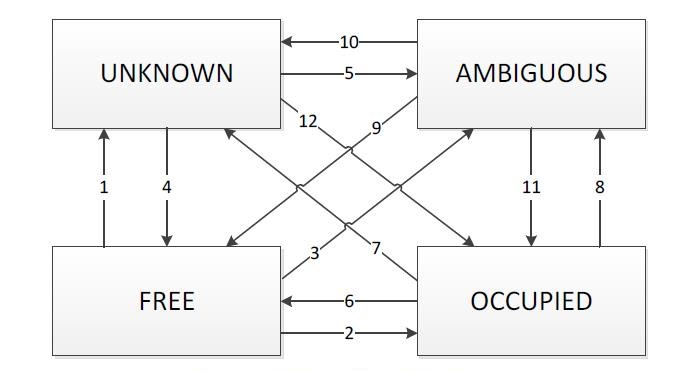
\includegraphics[width=0.8\textwidth]{fig3}
		\caption[Caption for LOF]{Status Transition among VSS. Figure from \cite{hybridl3}}
	\end{center}
  \end{figure}

  As is known by default, TTD has two states, free and occupied. And VSS can be regarded as a sub-section of TTD. As a prerequisite, no matter what is the status of VSS, free or occupied or ambiguous or unknown, TTD can be occupied. But if TTD is free, then all the VSS belongs to this TTD are all free. Following is a detailed explanation for each status transition \cite{hybridl3}. Since that, not all the status will be displayed later in the train model, only those status which are mentioned will be explained in details here. For the other status, please refer to Appendix 1.  

  \subsubsection{from free to unknown}

  As the VSS state becomes unknown, there must be at least one train located on the current TTD, in the rear of the current VSS. So the status of TTD should be occupied. In this case, several circumstances should be considered:

  \begin{itemize}
	
	\item
	
	There may be a disconnected train on the track, and there is no information about whether the disconnected train has moved to the next TTD. So the status of current VSS should be unknown, until time is up, or the current TTD is made sure to be free, or the train is finally connected.
	
	\item 
	
	The old VSS status (free) may be sent to a train which is occurring a communication failure by its Movement Authority (MA), and now the train is longer located in the old VSS, which it was reported. Due to the communication failure, the VSS status should be set to unknown.
	
	\item 
	
	If there exists disconnection between the train and trackside detection, then the status of VSS could not be supervised by a normal way. Since the train can still move to next VSS after disconnection, the current VSS status should be set as unknown as soon as the ``disconnect propagation timer'' expires, until the current TTD is known as free, or the train is reconnected, or the disconnected part is connected on the previous TTD.
	
	\item 
	
	Based on the above situation, there is also another possible reason that, the current VSS is not part of the MA, which means that, the current VSS has no idea about how the train is moving. So it should be unknown to the VSS if the train is located on it.
	
	\item 
	
	There is a situation, that the train loses its integrity accidentally. This action calls an ``integrity loss propagation timer''. As long as the integrity-lost train is still on the current TTD, once the timer expires, the status of the last reported VSS should be marked as unknown.
	
	\item 
	
	There may be a disconnected train on the track, and there is no information about whether the disconnected train has moved to the next TTD. A propagation timer is set for this disconnected train since it disconnects. Not until the timer expires will the VSS status be unknown.
	
  \end{itemize}	

  For more details of VSS status transition from free to unknown, please refer to the scenario described in chapter 4.3.6.

  \subsubsection{from free to occupied}

  \begin{itemize}
	
	\item 
	
	There is a train located on the current VSS, and the current status of the last VSS this train was reported is not unknown. As the train is moving in the right direction, the last VSS it was located in should also be reported with the status of ``occupied''.
	
	\item 
	
	If the train is moving from one TTD to the next TTD, and the TTD it has just left is now free, and the current VSS is the first VSS of the newly-entered TTD, then the VSS this train is currently located should be occupied.
	
  \end{itemize}	

  For more details of VSS status transition from free to occupied, please refer to the scenario described in chapter 4.2.1-4.2.7, and chapter 4.3.1-4.3.5.
  	
  \subsubsection{from free to ambiguous}

  \begin{itemize}
	
	\item 
	
	There is a train located on the current VSS, but the trackside detection is not possible to determine that whether there are any other trains located in the rear of this connected train or not. The train should have connection with the trackside detection, since that, if the train gets disconnected, the status may be ``unknown'' instead of ``ambiguous''.
	
	\item 
	
	If the train is moving from one TTD to the next TTD, and the TTD it has just left is now free, and the current VSS is the first VSS of the newly-entered TTD, then the VSS this train is currently located should be not free. And if the integrity status of the train is lost or no information available, which means that it is impossible to make sure of the train is integrate or not, then the VSS status should be ambiguous.
	
  \end{itemize} 

  For more details of VSS status transition from free to ambiguous, please refer to the scenario described in chapter 4.3.6-4.3.8.		

  \subsubsection{from occupied to free}

  \begin{itemize}
	
	\item 
	
	If there used to be a train located on the TTD, but now the train has left and TTD becomes free, then the current VSS also becomes free. Because that, information propagated from TTD is regarded as safe and trusted, which means that, TTD reports free, if and only if there is no train located on the current TTD. As a result, all VSS belong to this TTD can also be regarded as free.
	
	\item 
	
	If there is an integer train located on the VSS, then the VSS is occupied. When the integer train is reported to have left the VSS, then the status of the VSS is changed into free.
	
  \end{itemize}

  For more details of VSS status transition from occupied to free, please refer to the scenario described in chapter 4.2.2-4.2.7, and chapter 4.3.2-4.3.5.  

  \subsubsection{from occupied to unknown (see chapter 4.3.5)}

  \begin{itemize}
	
	\item 
	
	There must be train(s) located on the track, so VSS could be occupied. The current VSS is immediately turned into unknown as soon as the train located on the VVS disconnects from the trackside, which reveals that, there are still train(s) present, but due to disconnection, they cannot be detected. This may happen when the mute timer expires or it is end of a mission, which means the disconnection happens.
	
	\item 
	
	If an integer train is detected to be on the current VSS, then the status of the VSS is occupied. When the train has left the VSS, but meanwhile, it is reported as ``integrity lost'', or ``integrity information unavailable'', or train data has changed, then the status of the VSS should be changed. In this situation, the status of VSS should be set as unknown, since that, without having the integrity information of the train, it is unable to detect the location of the train, also the status of VSS. So the VSS, which is left by the train afterwards, should be set as unknown. The unknown state will be propagated until the disconnection timer expires or the train is reconnected or the whole TTD is confirmed to be free.
	
  \end{itemize}  

  For more details of VSS status transition from occupied to unknown, please refer to the scenario described in chapter 4.3.5.

  \subsubsection{from ambiguous to unknown}

  \begin{itemize}
	
	\item 
	
	If there is a train which is not integrated, and the train may be on this VSS, the status of this VSS is ambiguous. After all those trains have left this VSS, and this information has been reported by TTD, the status of this VSS becomes unknown.
	
	\item 
	
	If there is a train which is not integrated, and the train may be on this VSS, the status of this VSS is ambiguous. If the train is not leaving, which means that the train may still be on this VSS, but the mute timer for the train is expired, or it is time to the end of mission, which means that the current location and state of this train is not available. Then the state of the current VSS should be unknown.
	
  \end{itemize}  

  For more details of VSS status transition from ambiguous to unknown, please refer to the scenario described in chapter 4.3.7-4.3.8.  	

  The above are part of the detailed explanation of the state transformation among all the four states of VSS. In the next subchapters, a concrete example as the train model build in ABS language will be displayed and analyzed according to the above mentioned status. This will be shown as a further exploration of the concrete train model. To look for a integrate status transition of all possible situations, please refer to Appendix 1.
  

  \section{Details of the Train Model for Case Study I}
  
  Based on the Hybrid ERTMS/ETCS Level 3 Specification, three kinds of trains are described in this train model. The first one, also the most common one, is TIMS-equipped ERTMS train (also known as Integer train), which precisely occupies the exact VSS it is in. The next one comes the ERTMS train not fitted with TIMS, which occupies the sections in the rear of the track, until the end of the trackside detection section. The last type mentioned in this train model is non-ERTMS train, which occupies the whole trackside detection section as soon as it appears on the track.
  
  This chapter provides some details about the train model written in ABS language for case study I. Firstly it provides the design details of the mainly used interfaces in the model. Then it analyzes the model by comparing the above different types of train in order to verify the effectiveness of the process. At last it shows some extended discussion on the related properties of the model.
  
  \subsection{Introduction to the Basic Interfaces and Classes in the Model}
  
  Basically there are three interfaces in this train model --- interface Train, VSS and RBC. Interface Train contains a method move(), which manages the integrated movement of trains. For interface VSS and RBC, they have methods for describing the train moving and information propagating phases. Here is a detailed introduction of these two interfaces.
  
  \begin{itemize}	
  	
  	\item \textbf{interface VSS}
  	
  	Interface VSS is used to describe the behavior of a train when it leaves and arrives a VSS from the perspective of trackside. In interface VSS, there are four methods. The first two methods are designed for measuring TIMS-equipped ERTMS train (an integer train), while the other two methods are for ERTMS train not fitted with TIMS. 
  	
  	\begin{lstlisting}
  interface VSS {
  	Unit leaveTIMS(Int trainNo, VSS vss, Int leavePoint, Int arrivePoint) ;
  	Unit arriveTIMS(Int trainNo, Int arrivePoint) ;  		
  	Unit leaveNonTIMS(Int trainNo, VSS vss, Int breakPoint, Int arrivePoint) ;
  	Unit arriveNonTIMS(Int trainNo, Int arrivePoint) ;
  	}\end{lstlisting}
  	  	  	
  	Usually, a train should firstly leave a VSS, then it arrives the next VSS. The methods leave() and arrive() are just used to model this behavior. For the two leave() methods, both of them use two integer parameters to describe the leave point and arrive point of the train. While for the two arrive() methods, they should just remember the arrive point of the train, so only to mark the arrive point is enough. 
  	
  	\item \textbf{interface RBC}
  	
  	Interface RBC is used to act as a trackside management system. It collects all the information about the trains on the trackside, and propagates the information to the VSS and other trains. For example, if the first train, which is an integer train, steps onto the track, and keeps moving until it arrives VSS9, then VSS9 is occupied by the first train. RBC receives the information about the status change of VSS9, and reports the information to the next coming train, that the End of Authority for the next train should be VSS8. Here, End of Authority (EoA) is a location, it indicates the furthest VSS the current train can reach. If the former train stops at VSS9, and VSS1-VSS8 are all confirmed free, then the EoA for the current train should be VSS8. To decide every train's EoA in real time, as soon as they starts moving from the start point on the track, RBC plays an important role in managing all the information of the VSS status.
  	
  	\begin{lstlisting}
  interface RBC {
  	Unit connectRBCTIMS(Int trainNo, VSS vss, Int leavePoint, Int arrivePoint, RBC rbc, Map<Int, Status> map) ;
  	Unit connectRBCNonTIMS(Int trainNo, VSS vss, Int breakPoint, Int arrivePoint, RBC rbc, Map<Int, Status> map) ;
  	Int getnextEoA(RBC rbc, Int leavePoint, Int trainNo, Map<Int, Status> map) ;
  	Int getcurrentEoA(RBC rbc, Int leavePoint, Int trainNo, Map<Int, Status> map) ;
 	}\end{lstlisting}
  	
    Here in interface RBC, the method connectRBC() is used to connect the trackside(including the trains) and RBC in order to get information from each other. The information is basically collected from the movement of the trains, which has been recorded by calling the methods listed before, in interface VSS. Compared to those parameters mentioned above, methods in RBC holds two more parameters, those are RBC and Map<Int, Status>. RBC is regarded obviously as an object which stores all the information between trackside and RBC system, while the map is used to mark the change of the status for every VSS in order to decide the EoA for the next coming train. If an integer train passes VSS1 (which is initially marked as ``Free''), then the map of status for VSS1 stores in RBC would be changed from Pair(1,Free) to Pair(1,Occupied) to Pair(1,Free). Finally, if the next train wants to get its EoA from RBC, then it can just send a request to RBC to ask about where is the furthest “Free”. This is exactly how the method getEoA works.\cite{ayed2014b}

  \end{itemize}

  There are five classes in the train model. Three of them are just modeling three different kinds of trains, with interface Train being implemented.
  
  \begin{itemize}	
  	
  \item \textbf{class TrainTIMSImpl}
  
  Class TrainTIMSImpl implements interface Train, which contains a method move(). A TIMS-equipped ERTMS train, or an integer train, needs to call two methods to operate the movement of itself. These two methods are rewritten in move(). Firstly, it calls method leaveTIMS to simulate the leaving and arriving behavior of the train. After that, it reports the new states of the trackside and train itself to the RBC, then RBC stores the return result of method connectRBCTIMS(), in order to get and propagate the information, and also set the EoA for the next coming train. Class TrainNonTIMSImpl and class TrainNonERTMSImpl hold for a same idea. Here in this part, only class TrainTIMSImpl is explained in details as an example.
  
  \begin{lstlisting}
  class TrainTIMSImpl(Int trainNo, VSS leaveVSS, Int leavePoint, VSS arriveVSS, Int arrivePoint, RBC rbc, Map<Int, Status> map) implements Train {
  	Unit move() {  
  		Fut<Unit> fTIMS = arriveVSS!leaveTIMS(trainNo,leaveVSS,leavePoint,arrivePoint) ;
  		await fTIMS? ;
  		fTIMS.get ;
  		Fut<Unit> fRBC = rbc!connectRBCTIMS(trainNo,leaveVSS,leavePoint,arrivePoint,rbc,map) ;
  		await fRBC? ;
  		fRBC.get ;
  	}\end{lstlisting}
  \end{itemize}

  The other two classes are class VSSImpl and class RBCImpl, which implements interface VSS and RBC respectively.

  \begin{itemize}
  \item \textbf{class VSSImpl}
  
  Class VSSImpl implements interface VSS. It mainly simulates the movement of the train. As long as a train has not arrived its arrive point (which is exactly its End of Authority), it should move step by step, from one VSS to the next VSS. It should firstly leave the current VSS, then it calls method arrive() to make sure it arrives the next VSS. This behavior repeats until the train eventually arrives its EoA.
  
  Also, in order to manage the status change of TTD, here in this model, TTD is always regarded as a group of three VSS. This is enough for measuring the state of trackside, and also makes a simpler model to be realized.  
  
  \begin{lstlisting}
	class VSSImpl implements VSS {
		Unit leaveTIMS(Int trainNo, VSS vss, Int leavePoint, Int arrivePoint) {
			......
			if (leavePoint < arrivePoint) {
				leavePoint = leavePoint + 1 ;
			}
			Fut<Unit> fut1 = vss!arriveTIMS(trainNo,leavePoint) ;
			await fut1? ;
			fut1.get ;
			......
		}
		Unit arriveTIMS(Int trainNo, Int arrivePoint) {
			......
		}
		......
		//parts for NonTIMSTrain are omitted.
  }\end{lstlisting}

  \item \textbf{class RBCTIMSImpl}
  
  Class RBCImpl implements interface RBC. As introduced in interface RBC, class RBCImpl contains several methods which helps RBC system to receive and maintain the information from the train and trackside. After the operating behavior (leave and arrive) of the train, RBC is connected to the trackside and gets all such information stored in the RBC system. Once the status of a certain VSS changes, the map stored in RBC changes as well. Once the train passes a VSS, method getnextEoA() is called and RBC provides the result it stored to the parameter g of future type. As long as the train does not stop, method leave() and connectRBC() should run repeatedly, until the train arrives its final arrive point (EoA).
  
  \begin{lstlisting}
  class RBCImpl implements RBC {
  	Unit leaveTIMS(Int trainNo, VSS vss, Int leavePoint, Int arrivePoint) {}
  	Unit arriveTIMS(Int trainNo, Int arrivePoint) {}
  	......
  	Unit connectRBCTIMS(Int trainNo, VSS vss, Int leavePoint, Int arrivePoint, RBC rbc, Map<Int, Status> map) {
  		//RBC receives the information that there is a train occupying the current VSS.  
  		map = removeKey(map,leavePoint+1) ;        
  		map = insert(map,Pair(leavePoint+1, Occupied));
  		......
  		if (leavePoint < arrivePoint) {
  			leavePoint = leavePoint + 1 ;
 		}
  		......
  		//RBC receives the information that there is a train leaving the current VSS.  
  		map = removeKey(map,leavePoint-1) ;        
  		map = insert(map,Pair(leavePoint-1, Free));
  		//get EoA for the next train.
  		Fut<Int> g = rbc!getnextEoA(rbc,leavePoint,trainNo,map) ;
  		await g? ;
  		//If the train does not stop, then it goes on moving.
  		if (leavePoint < arrivePoint) {
  			Fut<Unit> l = this!leaveTIMS(trainNo,vss,leavePoint,arrivePoint) ;
  			await l? ;
  			Fut<Unit> c = this!connectRBCTIMS(trainNo,vss,leavePoint,arrivePoint,rbc) ;
  			await c? ;
  		}
  		......
  		//parts for NonTIMSTrain are omitted.
  }\end{lstlisting}

  \end{itemize}

  \subsection{TIMS-equipped ERTMS train (an integer train)}
  
  In the train model, the train comes first is an integer train, also known as TIMS-equipped ERTMS train. This kind of ERTMS train is fitted with TIMS, which means that it is responsible for its integrity. TIMS-equipped train use VSS to confirm the moving process and current situation of itself.
  
  In order to model this train, two interfaces are set up. One is interface VSS, which is used to confirm the situation of train according to the virtual fixed block it is located. The other one is interface RBC, which is used to implement the trackside system RBC to help propagate information between the train and the VSS.
  
  To make the model easier for understanding, it is set in this model that, every TTD is made up of 3 VSS. So it can be marked as, every 3 VSS are of the same TTD, and next 3 VSS are for next TTD. Since TTD has only two states, free and occupied, it is more complicated to confirm the status of VSS with four status (free, occupied, ambiguous, and unknown). As long as any VSS belong to this TTD is not free, TTD should be set as occupied. It is also much more convenient to have a fixed length of TTD in order to get an exact connection between the states of VSS and TTD. 
  
  To confirm the status of VSS and TTD, it is necessary to modify the moving phase of the train. To achieve this goal, method leave and arrive are used to control the behavior of the train and further its influence on the status of VSS and TTD, while method send and receive are used for RBC to get and propagate information from the train and to other VSS. Figure 5 shows a piece of sample code:
  
  \begin{figure}[H]
  	\begin{lstlisting}  	
  interface VSS {
  	Unit leaveTIMS(Int trainNo, VSS vss, Int leavePoint, Int arrivePoint) ;
  	Unit arriveTIMS(Int trainNo, Int arrivePoint) ;
  }  
  interface RBC {  
  	Unit connectRBCTIMS(Int trainNo, VSS vss, Int leavePoint, Int arrivePoint, RBC rbc, Map<Int, Status> map) ;  
  	Int getnextEoA(RBC rbc, Int leavePoint, Int trainNo, Map<Int, Status> map) ;
  	Int getcurrentEoA(RBC rbc, Int leavePoint, Int trainNo, Map<Int, Status> map) ;  
  }\end{lstlisting}
  	\caption[Caption for LOF]{Sample ABS code for the interfaces of TIMS-equipped ERTMS train.}
  \end{figure}
  
  The particular steps about the TIMS-equipped train's moving procedure is shown in Figure 6.
    
  \begin{figure}[H]
  	 \begin{center}
  	 	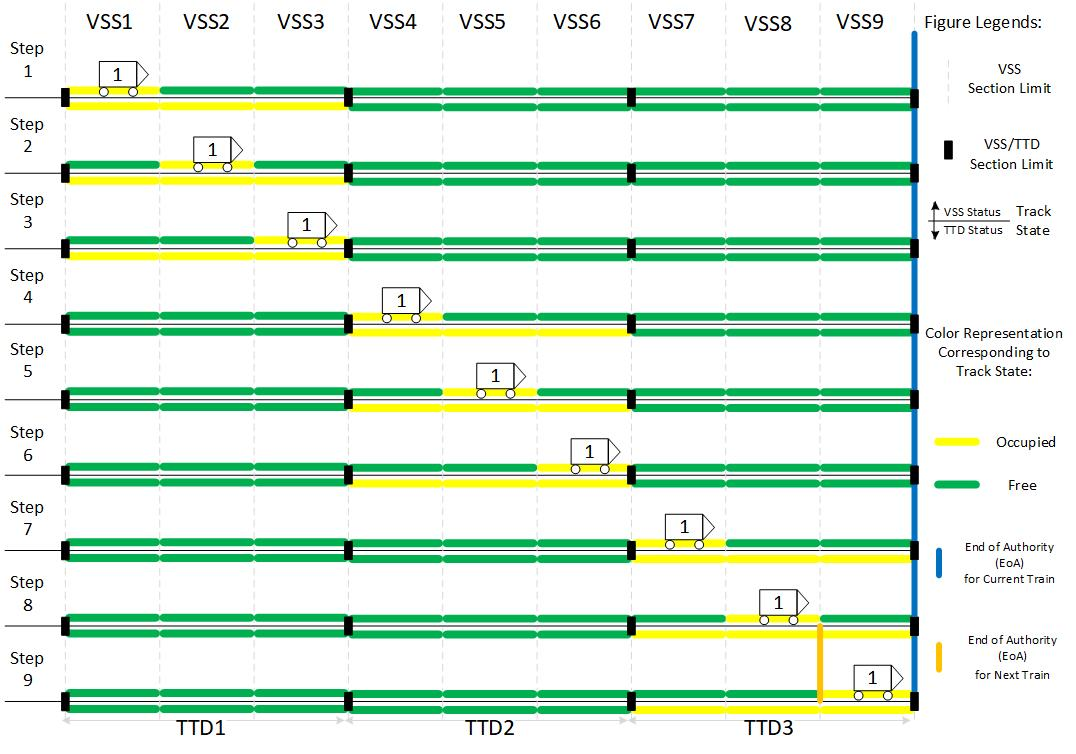
\includegraphics[width=0.8\textwidth]{train1}
  	 	\caption[Caption for LOF]{TIMS-equipped ERTMS train (an integer train).}
  	 \end{center}
  \end{figure}

  Train 1 in Figure 6 is a TIMS-equipped train. Here in the model in this situation, it holds its integrity all the time when it is moving. In this model, it is assumed that, all the trains are travelling in the same direction (from left to right in the figure) and in a straight line. Each TTD is made up of 3 VSS, and as shown in the figure, 3 TTD (9 VSS) are abstracted in this model. The EoA of the first train is set to the end point in the figure, which is VSS9.

  As shown in Figure 6, train 1 starts moving from VSS1, and stops at its End of Authority (EoA), which is VSS9. During its moving process, train 1 monitors the train integrity by itself as it is a TIMS-equipped train. The details of what happens and why it happens in each step are explained as follows:
  	
  	\subsubsection{Step 1}
  	
  	A TIMS-equipped train, train 1, enters the track. This changes the status of VSS1 from free to occupied, as mentioned above in the status transition. Since train 1 is located on TTD1, the state of TTD1 is turned into occupied from free. No changes to the other parts of the track.
  	
  	As soon as train 1 occupies VSS1, the trackside detection system RBC gets the information, that train 1 arrives and occupies VSS1. Then RBC sends this information back to the other VSS, informing the latest status of VSS1 and TTD1.
  	
    \subsubsection{Step 2}
  	
  	Train 1 is moving, it leaves VSS1, and arrives VSS2. This action makes the status of VSS1 from occupied back to free, and VSS2 from free to occupied. Since train 1 is still located on TTD1, the state of TTD 1 remains occupied.
  	
  	As train 1 is moving, the RBC is also receiving information from train 1. When train 1 leaves VSS1 and arrives VSS2, RBC receives this information, and sends back the changes in the state of VSS1 and VSS2 to the other VSS. The status of TTD 1 remains unchanged. 	
  	
  	\subsubsection{Step 3}
  	
  	Train 1 leaves VSS2, and keeps moving. Then it arrives VSS3, the last VSS of TTD1. Train 1 sends its information about its location to the trackside system RBC, and then RBC sends back the information it knows about the states of the track back to the VSS.
  	
  	In step 3, the integrate train 1 is on VSS3, VSS2 is no longer occupied, VSS3 is occupied instead. TTD1 is still occupied.
  	
  	Following shows a piece of the output for train 1 between VSS2 and VSS4.
  	
  	\begin{verbatim}
  	> ......
  	> Train 1 leaves VSS 2.
  	> VSS 2 is free.
  	> Train 1 arrives at VSS 3.
  	> VSS 3 is occupied by Train 1.
  	> RBC receives the information: Train 1 is now at VSS 3.
  	> RBC sends back the information: VSS 3 is occupied by Train 1. TTD 1 is occupied by Train 1. 
  	> VSS 2 is now free.
  	> Train 1 leaves VSS 3.
  	> VSS 3 is free.
  	> TTD 1 is free.
  	> ......
  	\end{verbatim}
  	
  	\subsubsection{Step 4-6}
  	
    This part is almost the same as step 1-3. So it is omitted.
  	
  	\subsubsection{Step 7}
  	
  	When train 1 leaves VSS6, the status of VSS6 becomes free again, at the meantime, the state of TTD2 also becomes free, since that there is no train on TTD2 any more. Then train 1 arrives VSS7, which makes the status of VSS7 to be occupied. TTD3 is also occupied. This information is also reported to RBC, and then propagated to other VSS by RBC.
  	
  	\subsubsection{Step 8}
  	
  	Train 1 leaves VSS7 and keeps moving. VSS 7 is free again. Once train 1 is detected to be arriving at VSS8, VSS8 is occupied. TTD3 is still occupied. All the information are reported to and from RBC.
  	
  	\subsubsection{Step 9}
  	
  	As is set at the beginning of the program, the End of Authority for train 1 should be VSS9, which means that, the farthest VSS that train 1 can arrive is VSS9. So after leaving VSS8 and arriving VSS9, train 1 should stop at VSS9, and sets the EoA for next train to VSS8, since VSS8 is the farthest VSS that the next train can arrive. Then it reports its location, the latest VSS status and the new EoA information to RBC. RBC then propagates this information back to the other VSS. The simulation of the movement of train 1 ends here. The final status of VSS1-VSS8, TTD1 and TTD2 are free, VSS9 and TTD3 are marked as occupied.
  	 	  
  \subsection{ERTMS train not fitted with TIMS}
  
  The second train in the model aims to show how an ERTMS train without TIMS works. If an ERTMS train is not fitted with TIMS, then it needs a limited amount of trackside detection to help with getting the information about the train data, and some separation operations as well.
  
  For the second train, when it enters the track, it is an integrate train with TIMS. But during its movement, the train splits into two parts, while the first half is able to go on moving as an integrate train, the second half acts as an ERTMS train with no TIMS any more. So for the latter, it is important to observe and model its states during movement along the track, in order to reflect the behaviors of an ERTMS train without TIMS.
    
  Here in the model, it is assumed that train 2 steps into the track also from VSS1. It keeps moving integrally on the track until it arrives VSS5, where it supposes to split into two parts, with the first half still integrated but the second half disconnected from the trackside. After the separation of the train, the first half of train 2 keeps moving to the subsequent VSS as an integer train, while the second half of train 2 is still disconnected. The status of each VSS should be measured according to the location of every part of train 2.
  
  For train 2, the interface VSS and interface RBC are still used, but with several extra methods. The measurement of the behavior of train 2 and the status of every VSS are classified into two parts: before separation and after separation of train 2. Because it should not be considered as an integer train before the separation, and the first part of train 2, which goes on moving after separation, can be reconsidered as an integer train to simulate. As a result, based on the first train which has been modeled above with interface VSS and interface RBC, a suitable model for train 2 is developed.
  
  A sketch of the model for train 2 could be like the above displayed program in Figure 7.
  
  \begin{figure}[H]
	\begin{lstlisting}
 Unit move() {
	 if(arrivePoint < 0) {
 		 arrivePoint = rbc.getcurrentEoA(rbc,leavePoint,trainNo,map) ;
 	 }
	 arriveVSS = new VSSImpl() ;
	 Fut<Unit> fTIMS = breakVSS!leaveTIMS(trainNo,leaveVSS,leavePoint,breakPoint) ;
	 await fTIMS? ;
	 fTIMS.get ;
	 Fut<Unit> fRBCTIMS = rbc!connectRBCTIMS(trainNo,leaveVSS,leavePoint,breakPoint,rbc,map) ;
	 await fRBCTIMS? ;
	 fRBCTIMS.get ;
	 //integrity loses
	 ......	
	 //integrity loss propagation timer starts
	 Time t = now() ;
	 await duration(1,1) ;
	 //connect RBC to make sure of the current EoA
	 Fut<Int> fEoA = rbc!getcurrentEoA(rbc,leavePoint,trainNo,map) ;
	 await fEoA? ;
	 fEoA.get ;
	 //integrity of the first half of Train 2 is confirmed
	 Fut<Unit> fNonTIMS = arriveVSS!leaveNonTIMS(trainNo,breakVSS,breakPoint,arrivePoint) ;
	 await fNonTIMS? ;
	 fNonTIMS.get ;
	 Fut<Unit> fRBCNonTIMS = rbc!connectRBCNonTIMS(trainNo,breakVSS,breakPoint,arrivePoint,rbc,map) ;
	 await fRBCNonTIMS? ;
	 fRBCNonTIMS.get ;   
 }\end{lstlisting}
	\caption[Caption for LOF]{Sample ABS code for the ERTMS train not fitted with TIMS.}
  \end{figure}
    
  The following Figure 8 shows the steps when the second train, which is without TIMS, is moving onto the track.
    
  \begin{figure}[H]
	\begin{center}
		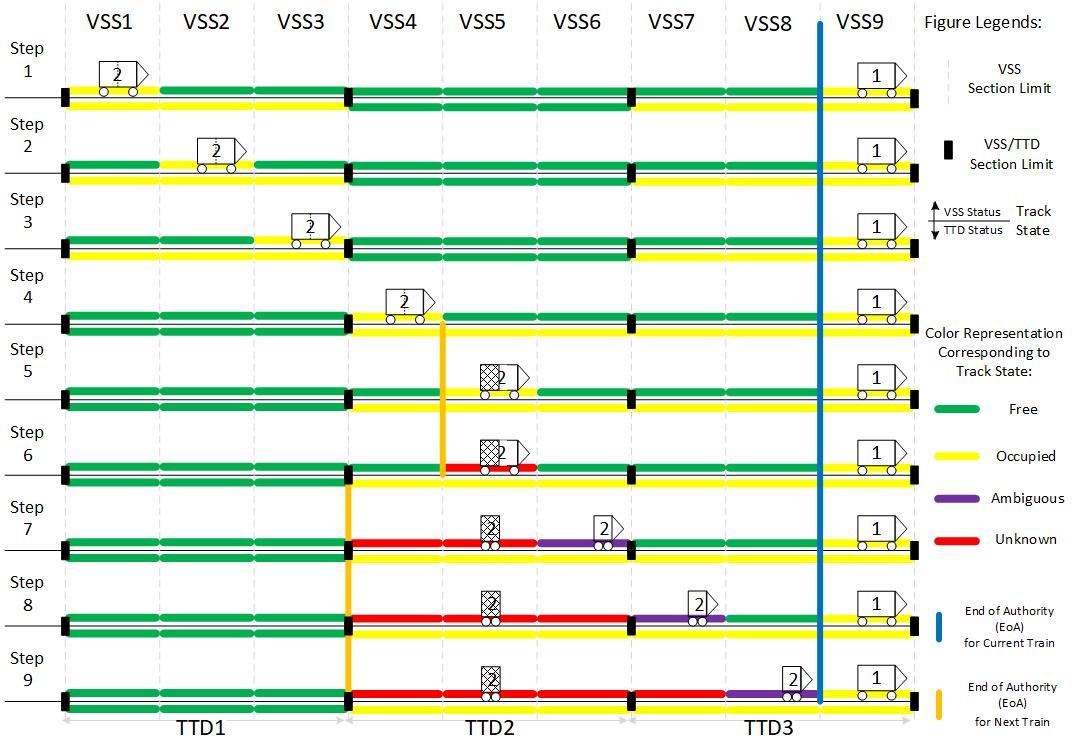
\includegraphics[width=0.8\textwidth]{train2}
		\caption[Caption for LOF]{ERTMS train not fitted with TIMS (the shadow part in the figure).}
	\end{center}
  \end{figure}

  The details of what happens and why it happens in each step are explained as follows:
	
	\subsubsection{Step 1}
	
    An ERTMS train not fitted with TIMS, train 2, enters the track. It should be noted that, train 1, which has stepped onto the track mentioned in the last part, is in front of train 2 and located on VSS9. The appearance of train 2 changes the status of VSS1 from free to occupied, as mentioned above in the status transition. Since train 2 is located on TTD1, the state of TTD1 is turned into occupied from free. No changes to the other parts of the track. 
    
    As soon as train 2 occupies VSS1, the trackside detection system RBC gets the information, that train 2 arrives and occupies VSS1. Then RBC sends this information back to the other VSS, informing the latest status of VSS1 and TTD1, which are both occupied.    
	
	\subsubsection{Step 2}
	
    Train 2 is moving, it leaves VSS1, and arrives VSS2. This action makes the status of VSS1 from occupied back to free, and VSS2 from free to occupied. Since train 2 is still located on TTD1, the state of TTD 1 remains occupied.
    
    As train 2 is moving, the RBC is also receiving information from train 2. When train 2 leaves VSS1 and arrives VSS2, RBC receives this information, and sends back the changes in the state of VSS1 and VSS2 to the other VSS. The status of TTD 1 remains unchanged, since train 2 is still on TTD1.

	\subsubsection{Step 3}
	
    Train 2 leaves VSS2, and keeps moving. Then it arrives VSS3, the last VSS of TTD1. Train 2 sends its information about its location to the trackside system RBC, and then RBC sends back the information it knows about the states of the track back to the VSS.
    
    In step 3, train 2 is on VSS3, VSS2 is no longer occupied, VSS3 is occupied instead. TTD1 is still occupied.
    
    \subsubsection{Step 4}
    
    Train 2 keeps moving. It leaves VSS3 and arrives at VSS4. It sends its location information to RBC, and RBC reports this information back to other VSS.
    
    It should be noticed that, since train 2 has left VSS3, TTD 1 and all VSS belongs to TTD1 are all free now.TTD 2 is now occupied.

    \subsubsection{Step 5-6}

    Train 2 stops at VSS5. This behavior is reported to RBC, and as a result, it also reports that the EoA for next train should be VSS4, as VSS4 is the last free VSS known to RBC. Then train 2 splits into two parts. The second half of train 2 is reported to lose its integrity, while the first half of train 2 still holds its integrity. According to the state transition specification introduced in chapter 4.1, the status of VSS5 becomes ambiguous due to the reported change for the integrity characteristic of train 2. Since the second half of train 2 loses its connection to the trackside, it is considered as remaining at VSS5 for now, while the first half of train 2 can still moving forward as an integer train.
    
    In step 6, when the first half of train 2 restarts moving, the status of VSS5 becomes unknown, since that it is unknown if the second part of train 2 is still at VSS5, or it moves as well. 
    
	\subsubsection{Step 7}
	
    As the first part of train 2 leaves VSS5, the status of VSS5 becomes unknown. According to the VSS state transition, since VSS4 is also part of TTD2, and TTD2 is now occupied by train 2, but it is unknown where the second part of train 2 is. So as the first part of train 2 moves forward, VSS 4 becomes unknown as well as VSS5. 
    
    When the first part of train 2 arrives at VSS6, the status of VSS6 is changed from free into ambiguous. The reason is that, the trackside RBC can get the information that the first part of train 2 is on VSS6, but it has no information about whether there is another vehicle (e.g. in this case, the second part of train 2 which has lost its integrity on VSS5.) in the rear of this first part of train 2 on the same VSS.
    
    It is also to be mentioned that, since VSS4 is now also reported as unknown, the latest EoA of the next train should be moved to VSS3.
    

    Following shows a piece of output for describing the influence train 2's behavior has over the status of the related VSS at its splitting point.
	
	\begin{verbatim}
	> ......
	> Train 2 arrives at VSS 5.
	> VSS 5 is occupied by Train 2.
	> Train 2 stops at VSS 5.
	> End of Authority for Train 3 should be VSS 4.
	> RBC receives the information: Train 2 is now at VSS 5.
	> RBC sends back the information: VSS 5 is occupied by Train 2. TTD 2 is occupied by Train 2. 
	> VSS 4 is now free.
	> Train 2 splits into 2 parts. The second half of Train 2 loses its integrity.
	> VSS 5 is now ambiguous because of Train 2.
	> The second half of Train 2 remains at VSS 5.
	> The first half of Train 2 leaves VSS 5.
	> VSS 5,4 are now unknown because of Train 2.
	> The first half of Train 2 arrives at VSS 6.
	> VSS 6 is ambiguous because of Train 2. TTD 2 is occupied by Train 2.
	> RBC receives the information: The first half of Train 2 is now at VSS 6.
	> RBC sends back the information: VSS 6 is ambiguous because of the first half of Train 2. 
	> TTD 2 is occupied by Train 2. VSS 5 is now unknown because of Train 2.
	> The first half of Train 2 leaves VSS 6.
	> VSS 6,5,4 are now unknown because of Train 2.
	> End of Authority for Train 3 should be VSS 3.
	> ......
	\end{verbatim}
	
	\subsubsection{Step 8}
	
	As the first part of train 2 keeps moving, it leaves VSS6 and heads to VSS7. It is not sure for RBC where exactly the first half of train 2 is, so VSS6 becomes also unknown. As a result, the whole TTD2 is occupied, while all the three VSS of TTD2 are unknown.
	
	When the first part of train 2 arrives at VSS7, the status of VSS7 becomes ambiguous, the reason is the same as mentioned before.
	
	\subsubsection{Step 9}
	
	Since train 1 stops at VSS9, and makes the EoA for train 2 be VSS8, the first half of train 2 arrives and stops at VSS8, with the status of VSS8 finally being ambiguous, and all VSS it passes after separation at VSS5 being unknown.
	
	To sum up, train 2 starts moving from VSS1, stops and splits at VSS5. After that, the second part of train 2 loses integrity, while the first part of train 2 keeps moving with integrity. Every VSS it arrives becomes ambiguous, and every VSS it then leaves becomes unknown, because of the unknown situation of the second part of train 2. The first part of train 2 finally stops at End of Authority, which is VSS8.  
  
  \subsection{non-ERTMS train}
  
  The third train comes onto the track is a non-ERTMS train. According to the definition of non-ERTMS train, it occupies the whole trackside detection when it enters the track. On the basis of the above results from train 1 and train 2, it is reported that, only TTD1 and the three VSS belong to TTD1 are free, which means that, once train 3 appears on the track, TTD1, as well as VSS1-3, are occupied.
  
  \subsection{Extended Discussion on the Properties}
  
  This chapter mainly provides some extended discussions on the properties of the model. For example, from the perspective of the deadlock analysis (SACO) and dynamic analysis (runtime behavior) will be discussed.
  
  \subsubsection{Deadlock Analysis}
  
  As is known to all, static analysis is a kind of technology for analyzing the program code without even running it, but just scanning the code with lexical analysis, syntax analysis, control flow analysis, etc., for the purpose of checking the properties like safety, reliability and maintenance of the program. Static analysis can help the developers find out some possible bugs existing in the code, and improve its correctness.
  
  Here for this train model building in ABS, it just needs to do the deadlock analysis as a sort of static analysis to check that if there are any deadlocks happening in the code. To do the deadlock analysis, there is no need to run the whole code, but just to use the Deadlock Analysis (SACO) toolkit. \cite{abstools}
  
  Usually, deadlock happens when there are more than two processes waiting for the same system resource, while the resource is currently occupied so no one can get the access to the resource. Whether there are deadlocks or not is a signal to tell the safety and reliability of a program. In best case, there should be no deadlocks, so that every process can be assigned to the needed resource as it wishes. In ABS, some kinds of deadlocks can be prevented from happening by using release points, type future is used to prevent deadlocks, since that future is used in asynchronous method calls to make sure that the current process awaits until the future is resolved. So, such as in the model, when using future, there is also an await in front of the get, which provides a release point for the method to be resolved in a sufficient period. Future, as a signal and value storage in asynchronous operations, is widely used to keep the program being deadlock-free. \cite{pachl2011deadlock}
  
  In the train model, future types are used in several situations. Following shows a detailed explanation with an example from the train model.

  In the class TrainTIMSImpl, to model the behavior of TIMS-equipped ERTMS train, the action of the train leaving and arriving every VSS should be simulated. A train should firstly leave the former VSS, then it is allowed to step into the next VSS. So there should be an asynchronous method call for the train of leaving and arriving the VSS. As shown in the following code segment, Fut<Unit> fTIMS is a future which stores the runnning result of method leaveTIMS into arriveVSS. While there is also a future Fut<Unit> f defined in method leaveTIMS to store the return value of method arriveTIMS into the current VSS to check that if the train has left this VSS. With the help of these two futures, the relative order of leaving and arriving of the train can be confirmed, which can, to some extent, ensure the safety and reliability of the model.

	\begin{lstlisting}  
  class TrainTIMSImpl(Int trainNo, VSS leaveVSS, Int leavePoint, VSS arriveVSS, Int arrivePoint, RBC rbc, Map<Int, Status> map) implements Train {
  	Unit move() {
  		Fut<Unit> fTIMS = arriveVSS!leaveTIMS(trainNo,leaveVSS,leavePoint,arrivePoint) ;
  		await fTIMS? ;
  		fTIMS.get ;
		......
  	}
  } 
  class VSSImpl implements VSS {
  	Unit leaveTIMS(Int trainNo, VSS vss, Int leavePoint, Int arrivePoint) {
  		......
  		Fut<Unit> f = vss!arriveTIMS(trainNo,leavePoint) ;
  		await f? ;
  		f.get ;
		......
  	}
    Unit arriveTIMS(Int trainNo, Int arrivePoint) {
  		......
  	}
  }  \end{lstlisting}
  
  In order to statically tell if there are deadlocks in the ABS program, the Deadlock Analysis (SACO) toolkit is used along with the future type in the program. On the basis of the theoretical explanation presented above, the result of Deadlock Analysis (SACO) also shows that, there is no deadlock in the train model program.
  
  \begin{verbatim}
  > Pointsto analysis performed in 3 ms.
  > LMhp analysis performed in 0 ms.
  > Mhp graph created in 1 ms.
  > Closure time 0 ms.
  > Discarded 0 cycles with freshness analysis.
  >
  > The program is deadlock free
  >
  > Complete analysis performed in 4 ms.
  \end{verbatim}
  
  It turns out that the model built for this case study is deadlock free. As a result, the train model is safe according to deadlock analysis.
  
  
  \subsubsection{Dynamic Analysis}
  
  Once using the online collaboratory to run ABS programs, the Simulator (Erlang) is the main and effective tool to do simulation for ABS models. The Erlang Simulator uses type checker as compiler frontend to generate Erlang code to be compiled on the Erlang BEAM VM, and it uses a compiler backend to generate Erlang application. \cite{abstools}
  
  By using this Erlang Simulator of online collaboratory, the train model could be checked and run. It can be inferred from the output result that, if there exists any problem. For example, by printing out the map stored in RBC within each phase, it is possible to find out if the map is modified incorrectly, or if there is a part being omitted.
  
  After time to time modifying and testing, the model runs smoothly in the end, which provides a reasonable result of the simulation of the model.
  
  
  
  \section{Case Study II: }
  
  \section{Discussion and Evaluation}
  
  \section{Related Work}
  
  
  
 
  
  \appendix
  \appendixpage
    
\renewcommand\refname{Appendix}
%\bibliographystyle{plain}
%\bibliography{Appendix}

  \section{Details of Status Transition}

  In this chapter, the remaining status which have not appeared in the above train model, are further explained as follows:

  \begin{itemize}
	
	\item \textbf{from unknown to free.}
	
	\begin{itemize}
		
		\item 
		
		Since the initial state of VSS is unknown, as long as it is confirmed that the current TTD has no train located on it, the current status of VSS is obviously free.
		
		\item 
		
		There is an integer train which loses its connection to the trackside detection, but reconnects at the same point. For this train, when its integrity is lost, the status of the VSS it is located becomes unknown. Then after reconnection, the VSS in advance of the train, which is also part of the original MA, becomes free.
		
		\item 
		
		There is an integer train which loses its connection to the trackside detection, but reconnects at the same point, and no change happens on the train data (including length). For this train, when its integrity is lost, the status of the VSS it is located becomes unknown. Then after reconnection, the VSS in the rear of the train, which is also part of the original MA, becomes free. And also, the subsequent VSS are still unknown at first, since the VSS, on which the connection-lost train is located, is free now.
		
	\end{itemize}  	
	
	\item \textbf{from unknown to ambiguous.}
	
	\begin{itemize}
		
		\item 
		
		Due to disconnection or propagation of a train, the current status of VSS is unknown. So it is confirmed that there is at least one train on the track. But it is impossible for the trackside to confirm that if there are any other trains or vehicles located in the rear of a connected train. So the status of current VSS is turned into ambiguous.
		
	\end{itemize} 
	
	\item \textbf{from occupied to ambiguous.}
	
	\begin{itemize}
		
		\item 
		
		If an integer train is detected to be on the current VSS, then the status of the VSS is occupied. When the train has left the VSS, but meanwhile, it is reported as ``integrity lost'', or ``integrity information unavailable'', or train data has changed, then the status of the VSS should be changed. In this situation, the status of VSS should be set as ambiguous, since that, without having the integrity information of the train, it is unable to detect the location of the train, also the status of VSS. And since the VSS is the train currently located on, the status of the current VSS should be ambiguous.
		
		\item 
		
		VSS is at first occupied, since at least one train is confirmed on the current VSS. If the VSS in the rear of the current VSS are all set to unknown, for example, when the train reconnects to the trackside detection, the VSS rearwards become unknown. If so, when the train leaves the current VSS, this VSS should be set as ambiguous, since that it is not possible for the trackside detection to get the information that whether there are other trains or vehicles in the rear of a connected train.
		
		\item 
		
		If there is another train also located on the VSS, but the trackside detection is not able to confirm that, then the status of the VSS should be set to ambiguous.
		
	\end{itemize}  
	
	\item \textbf{from ambiguous to free.}
	
	\begin{itemize}
		
		\item 
		
		Once the TTD information is confirmed, the status of TTD is regarded as trustable. So, if the TTD information reports that there is no train on the current track, then all the VSS belong to this TTD are also considered as free.
		
		\item 
		
		There may be a train, which has a vehicle rearwards. The vehicle may be either an exact train but without any connection to the trackside, or a virtual train which may lead to the ambiguous state of VSS, then this vehicle is considered as a shadow train. If the first train has already left the first VSS, the following VSS should be ambiguous because of the undetected shadow train. But after the detecting timer expires, these VSS can be reset to free.
		
	\end{itemize}
	
	\item \textbf{from ambiguous to occupied.}
	
	\begin{itemize}
		
		\item 
		
		If there is a shadow train on the track, the trackside cannot detect it and starts a timer. Then, the status of the current VSS is ambiguous before the timer expires. Even though the shadow train may be leaving, as long as the leaving distance is shorter than the distance this train can move during the timer, the VSS status is still ambiguous. Once an integer train is reported on the current VSS after that, the status of the VSS should be occupied.
		
		\item 
		
		If there is a shadow train on the track, the trackside cannot detect it and starts a timer. Then, the status of the current VSS is ambiguous before the timer expires. If the TTD in the rear of the current train is free, and the current integer train on the same VSS has left the last TTD, then the current VSS should be occupied as the integer train is reported.
		
	\end{itemize}    	
	
	\item \textbf{from unknown to occupied.}
	
	\begin{itemize}
		
		\item 
		
		If there is an integer located train on a VSS, then the current TTD should report occupied. If the train disconnects and then reconnects within the same session with all the train data unchanged, then the current VSS should change its status from unknown (disconnection) to occupied (reconnection). As the same time, all the subsequent VSS also become unknown since that, once the train loses its connection, there is an integer train located on an occupied TTD, so the status of the rest VSS become unknown.
		
		\item 
		
		If there is an integer located train on a VSS, then the current TTD should report occupied. If the train disconnects from the trackside, then the current VSS becomes unknown. But as the train is still moving, once it arrives the next VSS, but that VSS has not received the disconnected information about the integer train, then this VSS will be considered as occupied first.
		
	\end{itemize}
	
  \end{itemize}

\renewcommand\refname{Reference}
\bibliographystyle{plain}
\bibliography{reference}

\end{document}
